% vim: spell spelllang=en:
%! TEX root = **/00-main.tex

% Hierarchical Clustering on original data:

\section{Hierarchical Clustering}%
\label{sec:hierarchical_clustering}

% TODO:

% Precise description of the data used (which variables have not been included
% in the analysis, if any, whenever you are using a CURE strategy, provide
% details about eventual sampling performed on data, etc)

% Clustering method used, metrics and aggregation criteria used (Ward’s method
% is recommended embedded or not in a CURE strategy whenever scaling to big data
% is required, for messy data Gower dissimilarity coefficient to the square is
% recommended )

\begin{landscape}

\subsection{Dendogram}%
\label{sub:dendogram}

% Resulting Dendrogram (of the total dataset or the sample). USE A SINGLE PAGE
% for it

\begin{figure}[H]
    \centering
    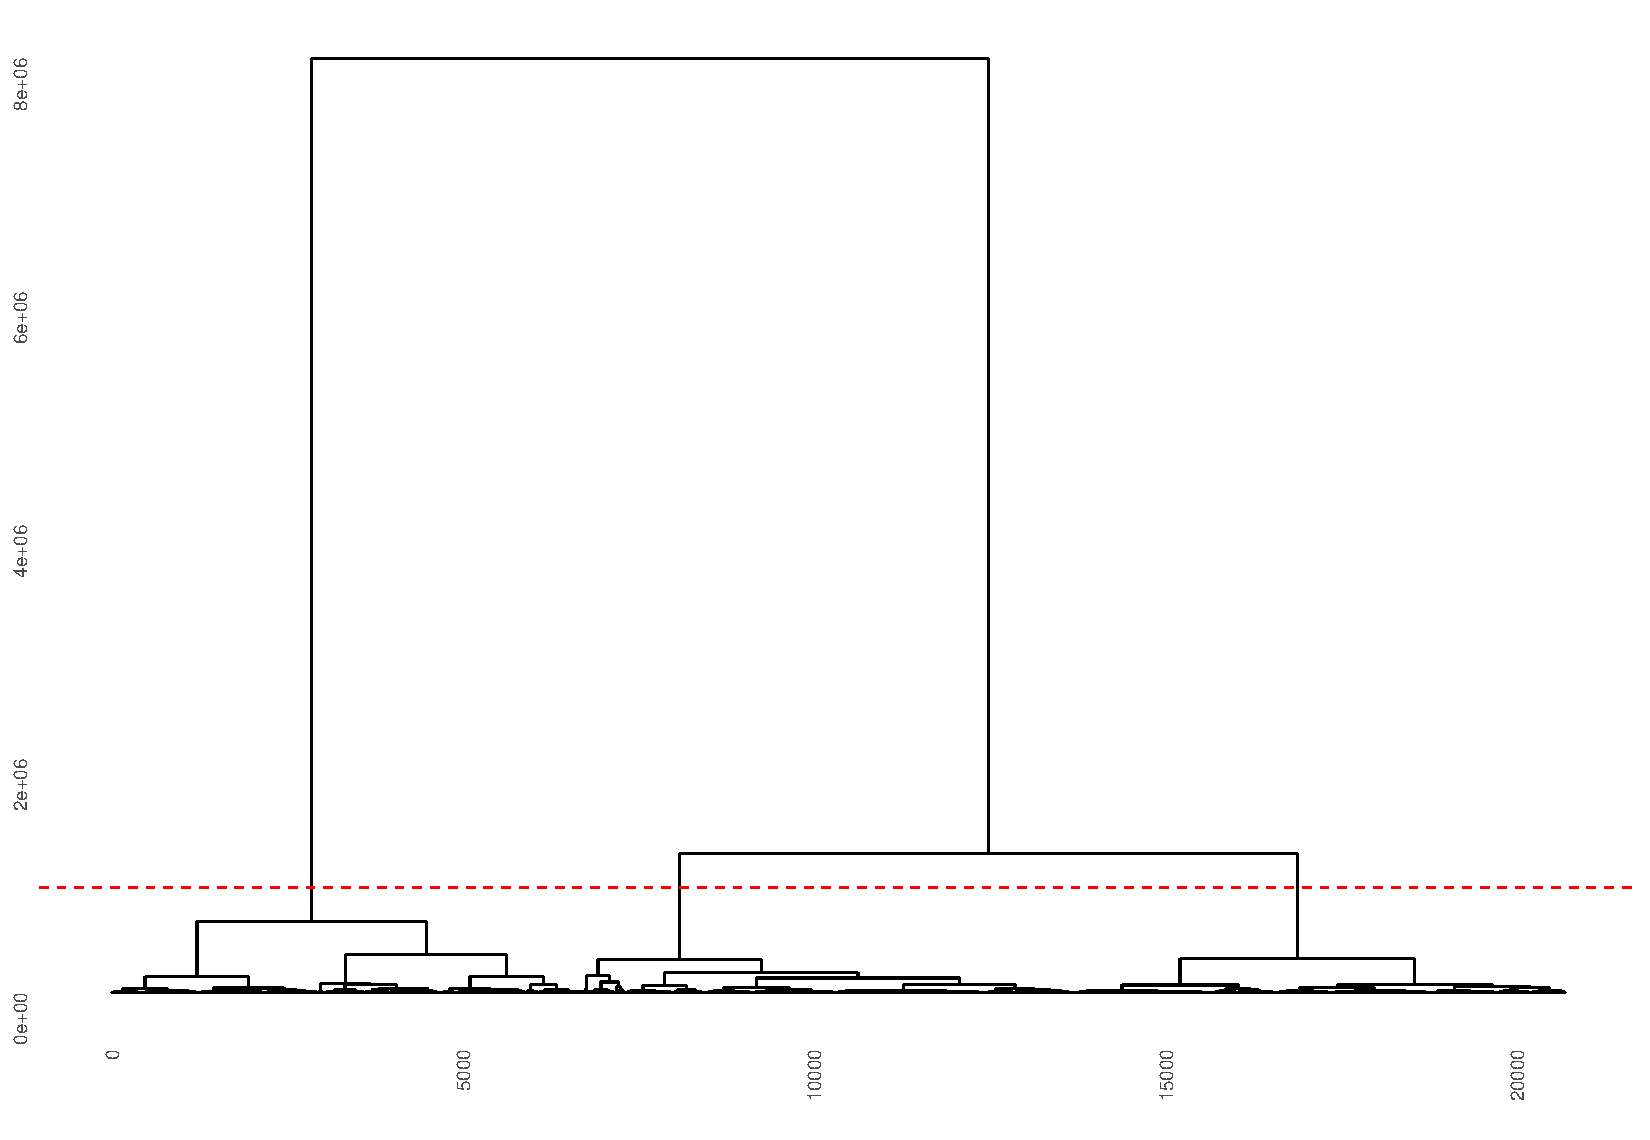
\includegraphics[width=0.8\linewidth]{dendogram}
    \caption{Cluster Dendogram}%
    \label{fig:dendogram}
\end{figure}

\end{landscape}

% Discuss about how to get the final number of clusters

\subsection{Description of clusters}%
\label{sub:description_of_clusters}



% Table with a description of the clusters size
